\documentclass[letterpaper]{article}

\title{Diversity in Computer Science}
\date{Friday March 18th, 2016}
\author{Michael McRoskey - mmcrosk1@nd.edu}

\usepackage{graphicx}
\usepackage{hyperref}
\usepackage[section]{placeins}
\usepackage[margin=1in]{geometry}
\usepackage{indentfirst}

\begin{document}

\maketitle
%-----------------------------------------------
\section*{Overview}

Having raw data on the ethnic makeup of computer science students at Notre Dame was really helpful because it allowed me to visualize how the campus climate is changing (or not) with respect to gender and ethnicity. To process this data, I used awk to:

\begin{itemize}
	\item Create column arrays of the different years
	\item Use the size of those arrays to calculate class size
	\item Manually print calculated percentages for each group
\end{itemize}

I used {\tt data.sh} for the awk commands and {\tt plot.plt} to generate line graphs representing the percentage change over time.

%-----------------------------------------------
\section*{Methodology}

\subsection*{Processing Demographics}

{\tt data.sh} pipes {\tt demographics.csv} into the awk command and counts the data in each column with the format {\tt s2013[\$1]++} where {\tt s} represents sex and {\tt r} represents race/ethnicity for each year. 

The {\tt END} block adds the M and F numbers to get a total class size for each year. I had to make sure that blank parts of the CSV file evaluated as {\tt false}. Finally, I printed results in a terribly inefficient yet effective manner:
 
	\begin{verbatim}
	# 2013 Results
		print "2013,", s2013["M"]*100/tot2013, ",", s2013["F"]*100/tot2013, ",", r2013["C"]*100/tot2013, ",", r2013["O"]*100/tot2013, ",", r2013["S"]*100/tot2013, ",", r2013["B"]*100/tot2013, ",", r2013["N"]*100/tot2013, ",", r2013["T"]*100/tot2013, ",", r2013["U"]*100/tot2013
	\end{verbatim}

All of this printing gets redirected to {\tt data.csv}, which is used in {\tt plot.plt}.

I think the most frustrating part was figuring out how to restructure the data. Because I was dealing with so many years, I wanted to nest my statements in for loops going from 2013 to 2018. However, I also wanted to utilize some of the abstraction of associative arrays. Ultimately, my solution wasn't pretty and required a lot of copy and paste, but it worked.

\subsection*{GNU Plot}

{\tt plot.plt} formats GNU plots {\tt race.png} and {\tt sex.png} by outputting a PNG line graph with the proper labels. I had to make sure that the percentage values in {\tt data.csv} were multiplied by 100 so that the plot could handle the axes appropriately.

 
%-----------------------------------------------
\section*{Analysis}

I was surprised at the statistical disparity between men and women students in Notre Dame Computer Science. The lines were not very close to an equitable 50\% and are fairly flat. However, there was a slight trend toward convergence in recent years. It was a good decision to use a percentage because that reflects proportion rather than pure numbers, which can be difficult to judge.

\begin{figure}[!htb]
\centering
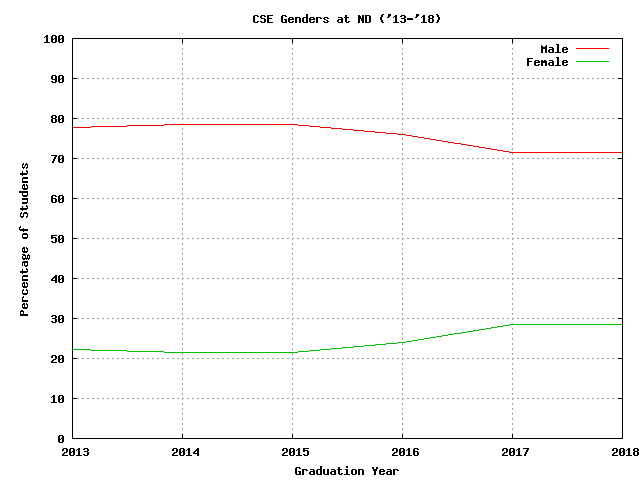
\includegraphics[width=5in]{sex.png}
\caption{Gender Disparity in Notre Dame Computer Science}
\label{fig:gender}
\end{figure}

Figure 2 shows a no definable trend in recent years but a significant proportion of Caucasian students in Notre Dame Computer Science. Although there isn't a great line of best fit for other ethnicities, it's for certain that they remain well under 20\%, even 10\%.

\begin{figure}[!htb]
\centering
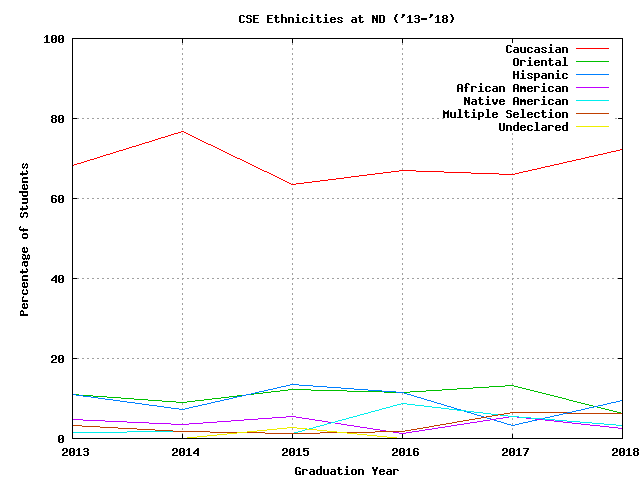
\includegraphics[width=5in]{race.png}
\caption{Ethnic Diversity Disparities}
\label{fig:race}
\end{figure}

The results of the outputted {\tt data.csv} file:

\begin{table}[h!]
    \centering
    \begin{tabular}{l|c|c|c|c|c|c|c|c|c}
    Year & Male & Female & Caucasian & Oriental & Hispanic & Black & Native-Am & Mult. & Undeclared\\
    \hline
    2013 & 78 & 22 & 68 & 11 & 11 & 5 & 2 & 3 & 0\\ 
    2014 & 79 & 21 & 77 &  9 &  7 & 4 & 2 & 2 & 0\\
    2015 & 78 & 22 & 64 & 12 & 14 & 5 & 1 & 1 & 3\\
    2016 & 75 & 25 & 67 & 11 & 11 & 1 & 9 & 2 & 0\\
    2017 & 71 & 29 & 66 & 13 &  3 & 5 & 5 & 7 & 0\\
    2018 & 71 & 29 & 72 &  6 & 10 & 2 & 3 & 6 & 0
    \end{tabular}
    \caption{Percentages of Groups}
    \label{tbl:example}
\end{table}

%-----------------------------------------------
\section*{Discussion}

\subsection*{Notre Dame's Ethnic Makeup}

I think it's really important to pay attention to our ethnic makeup. I saw "Decoding the Gender Gap" this year, a really compelling documentary that explores these demographic disparities in computer science. I understand the need to promote diversity so that there can be a broader range of ideas for a broad range of humanity, especially in a profession where lines of code affect millions of users. I think it's also important to understand Notre Dame's core ethnic makeup, since we're predominantly Caucasian. I would love to find out statistics from our institution on ethnicity overall, because I think it will likely be the same type of results: vast disparities. That would lead me to conclude that this is not necessarily a departmental concern, but a University-wide one, although departmental efforts to broaden exposure never hurts.

\subsection*{Ways to Improve Notre Dame's CSE Diversity}

Computer Science seems to be one of the fastest growing majors across the country. I think we need to tap into that and lure more talented students into the program, which could certainly help our diversity. I think there should be an Intro to Computer Science Course as offered at some of our peer institutions open to all first year students across all majors.

Although I have never felt unwelcome, intimidated, or outnumbered in computer science, I understand students who could feel this way. I think it's important for us all to "be in it together" and I appreciate the effect group projects have on this front. I've always felt a sense of belonging and want to make sure other students feel this way too.

\end{document}

